\subsection{Correção do Gap devido a movimentação da bola}

Somente o ajuste de movimentação da bola foi anulado. Os resultados
no planejamento são apresentados na figura~\ref{fig:kickpos_0}.

\begin{figure}[H]
  \centering
  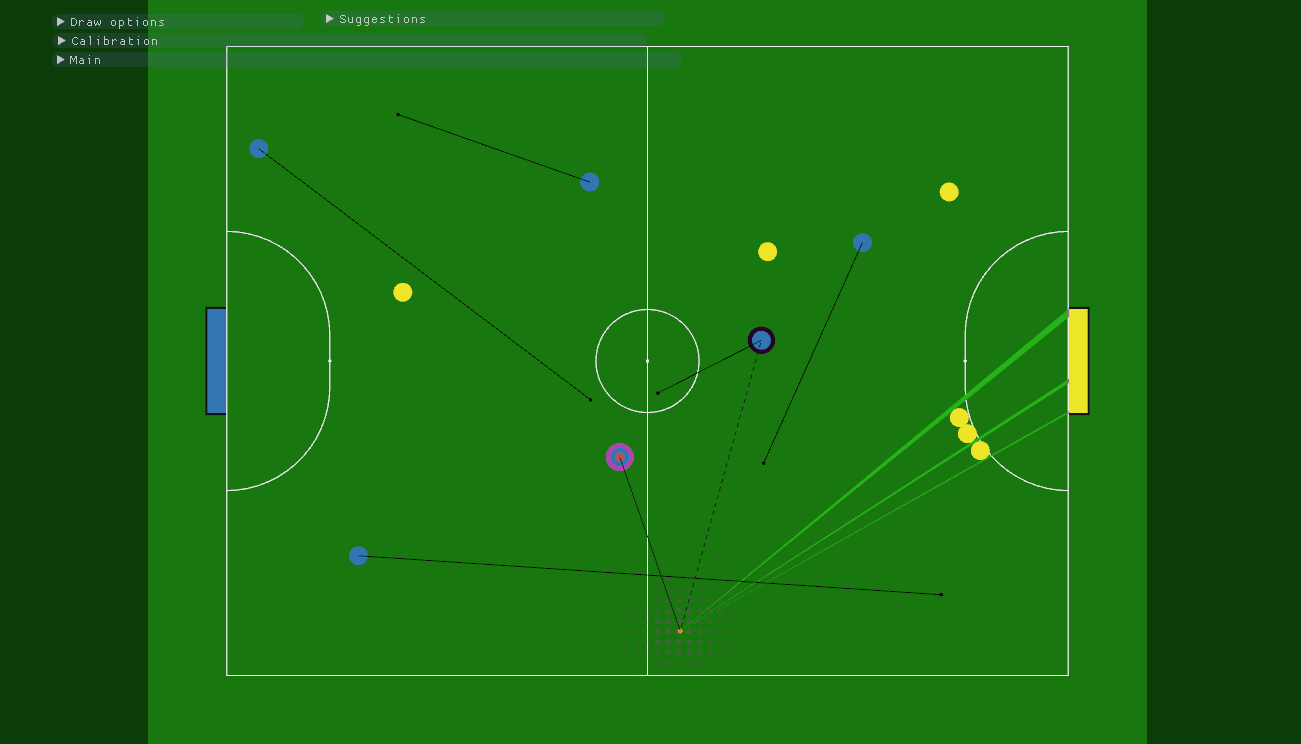
\includegraphics[width= 0.8\linewidth]{result/kickpos_0_atq}
  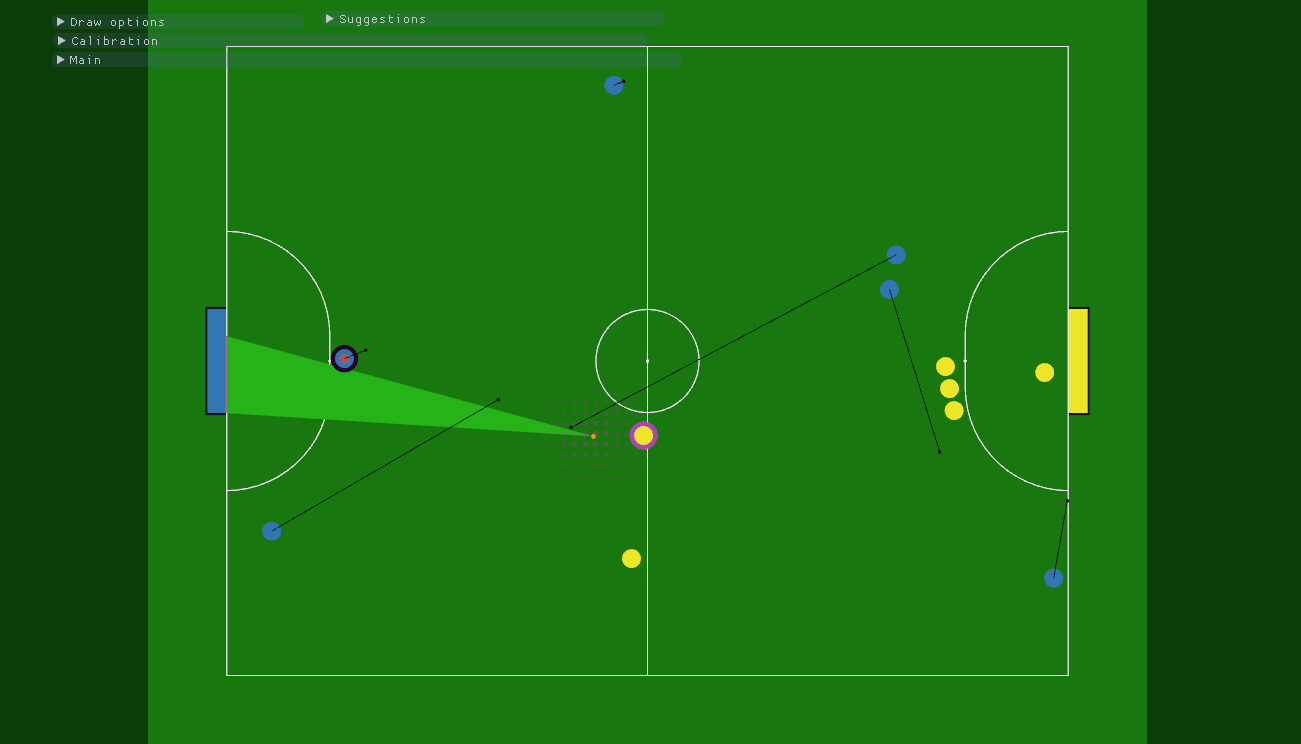
\includegraphics[width= 0.8\linewidth]{result/kickpos_0_def}
  \caption{Planejamento com os parâmetros inicias e o sem ajuste
           de movimentação da bola em ambiente de
           ataque (acima) e defesa (abaixo)}\label{fig:kickpos_0}
\end{figure}

Depois esse ajuste foi alterado para $0.24$. Os resultados 
em ambiente de ataque e defesa são apresentados na
figura~\ref{fig:kickpos_024}.

\begin{figure}[H]
  \centering
  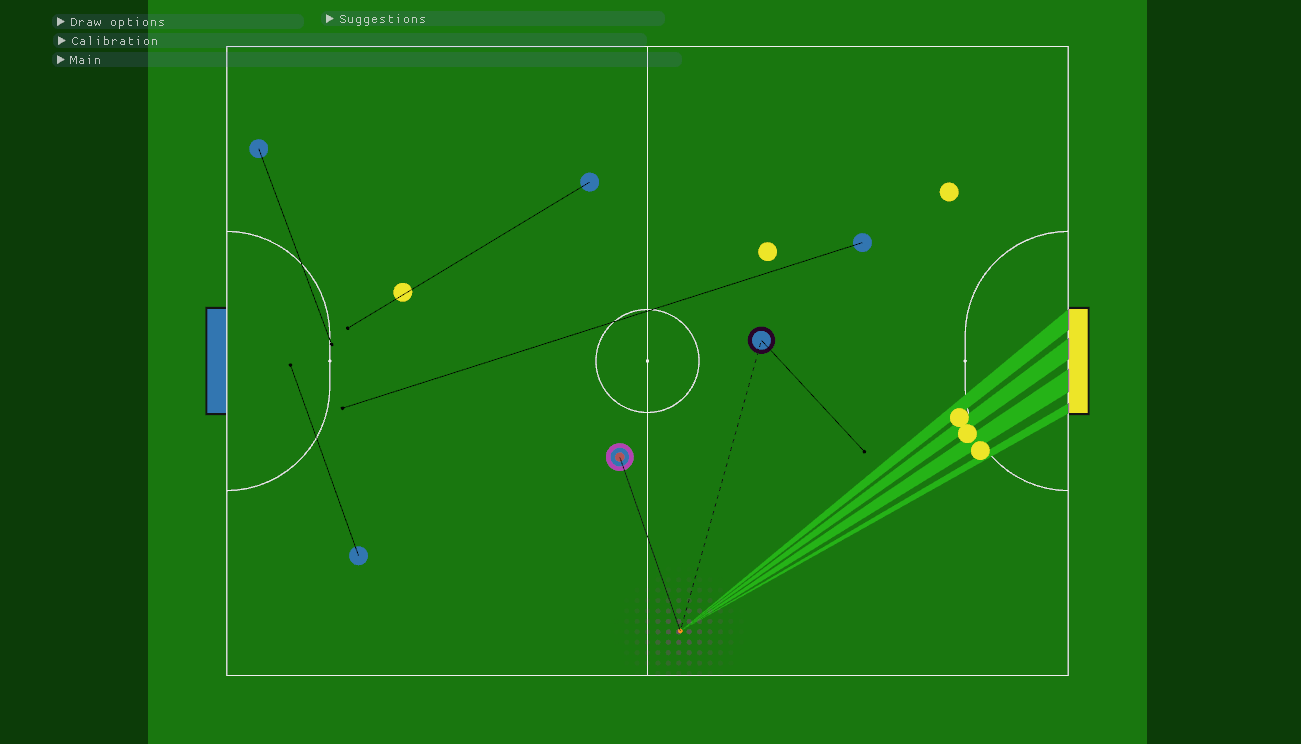
\includegraphics[width= 0.8\linewidth]{result/kickpos_024_atq}
  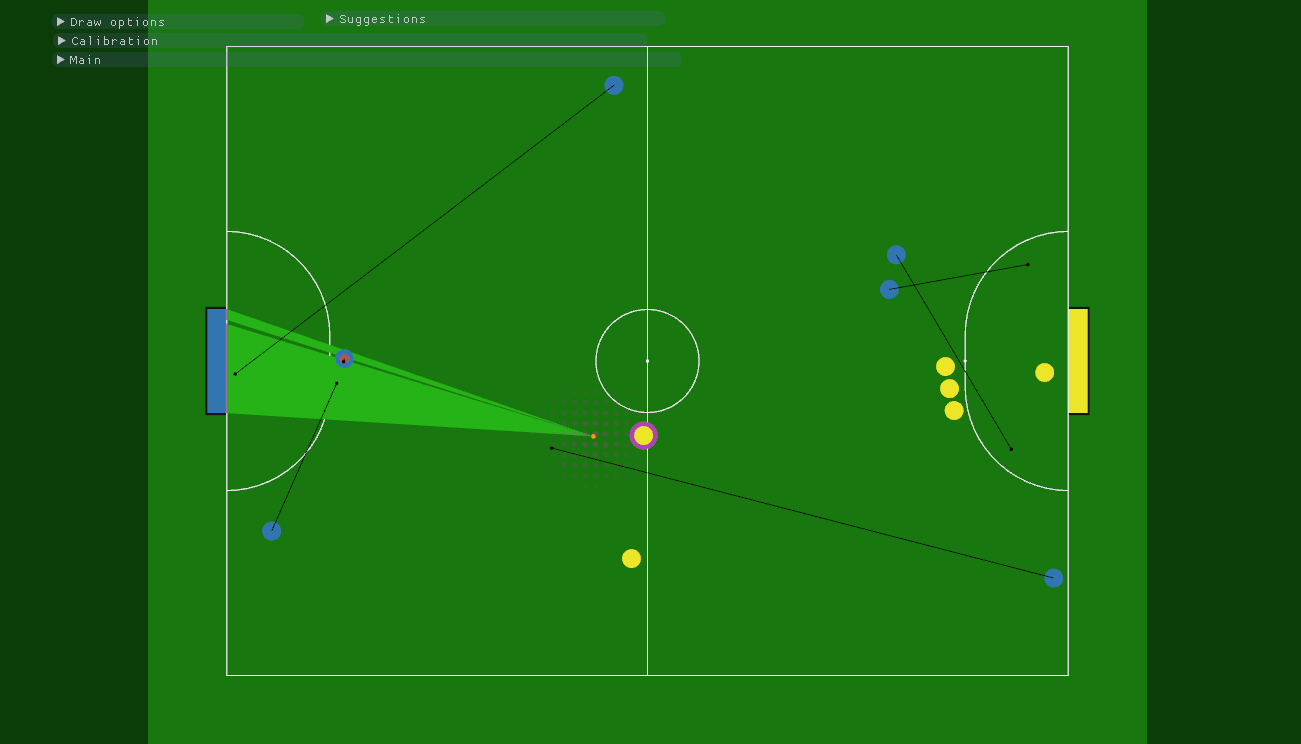
\includegraphics[width= 0.8\linewidth]{result/kickpos_024_def}
  \caption{Planejamento com os parâmetros inicias e o ajuste de
           movimentação da bola ajustado para $0.24$ em ambiente de
           ataque (acima) e defesa (abaixo)}\label{fig:kickpos_024}
\end{figure}
